\section{Anexos de la Práctica 5}
\begin{figure}[ht!] % 'h' indica que la imagen se coloca aquí
    \centering
    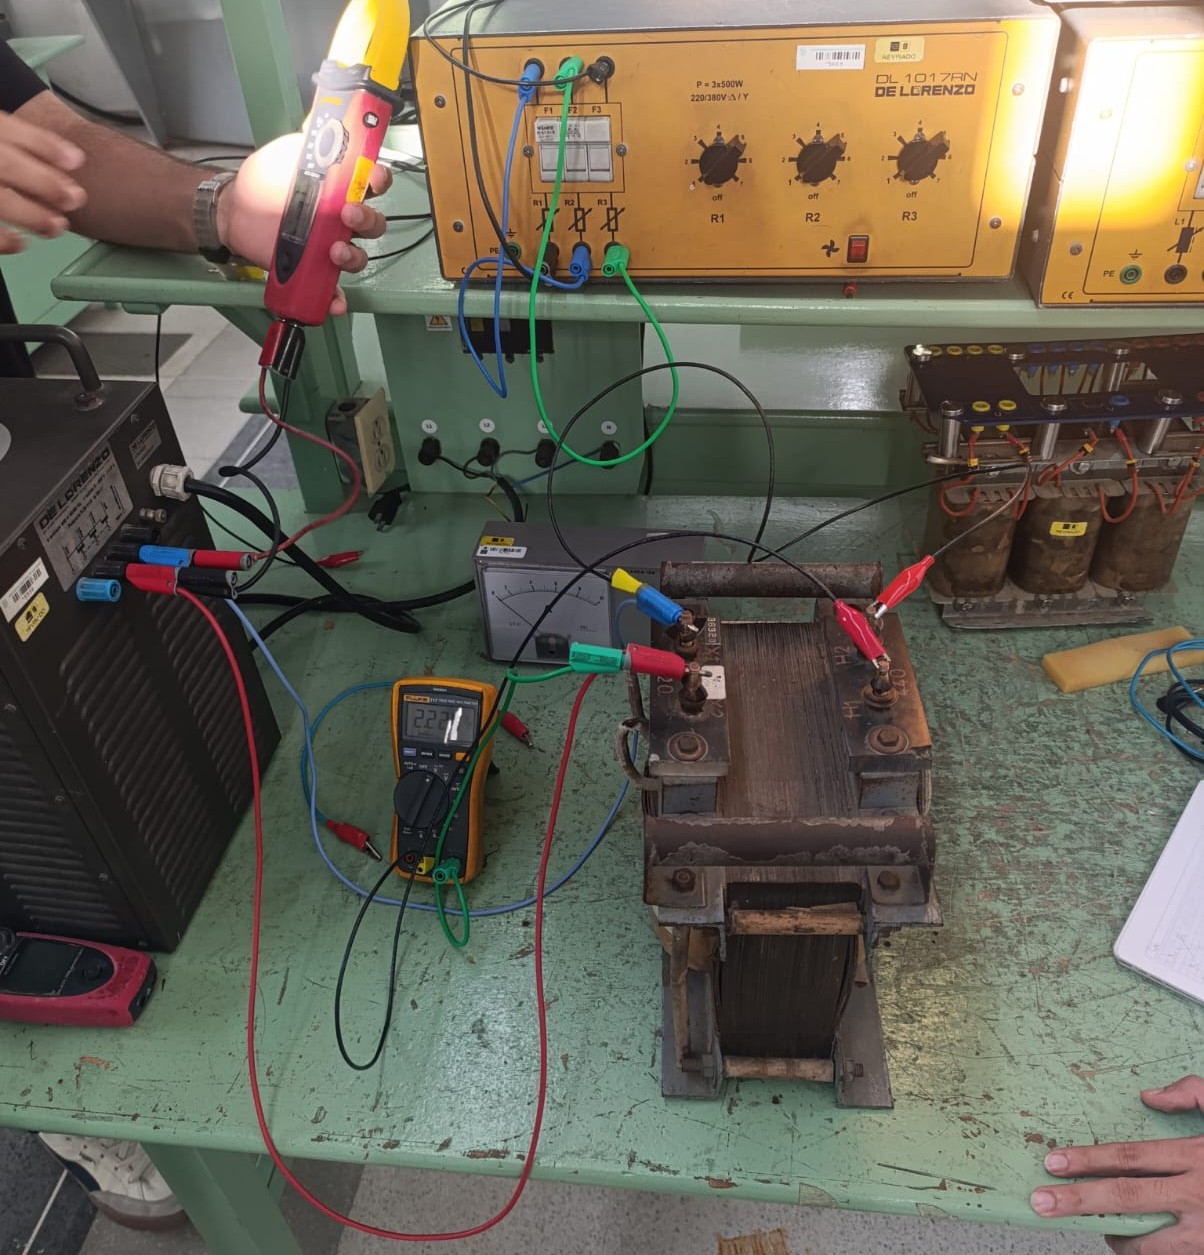
\includegraphics[width=0.48\textwidth]{fot/prac4_autoenvacio.jpeg} % Cambia la ruta a tu imagen
    \caption{Autotransformador en la prueba de vacio (Hay una carga de resistencias en serie que estan desconectadas).}
    \label{fig:prac4_autoenvacio}
\end{figure}

\begin{figure}[ht!] % 'h' indica que la imagen se coloca aquí
    \centering
    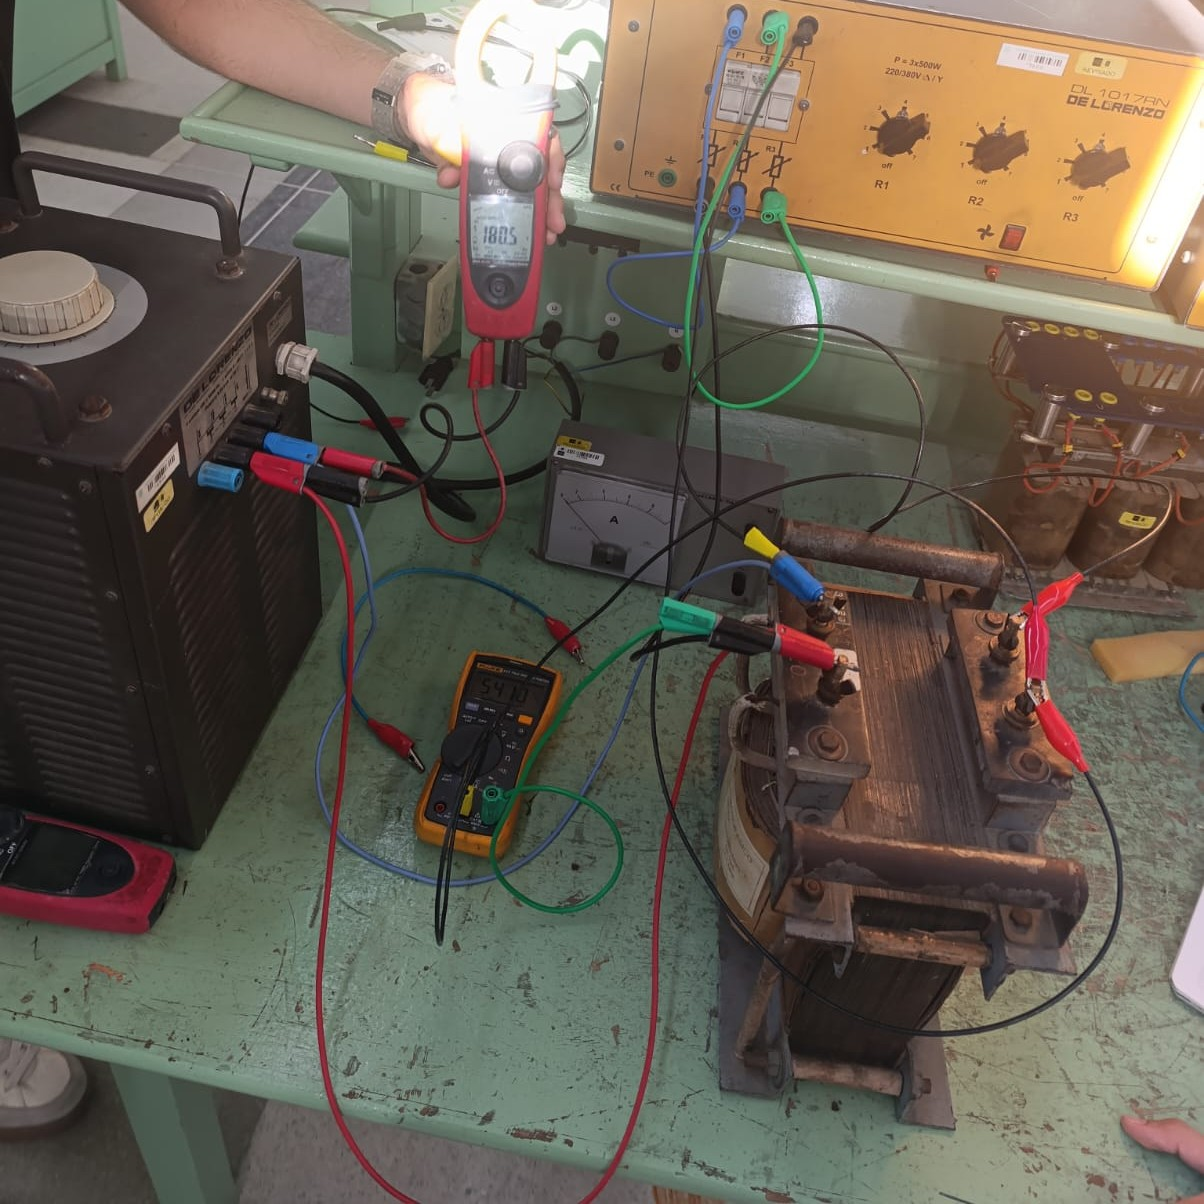
\includegraphics[width=0.48\textwidth]{fot/prac4_autoR_.jpeg} % Cambia la ruta a tu imagen
    \caption{Autotransformador con tres cargas resistivas conectadas en serie.}
    \label{fig:AutoR1}
\end{figure}